\documentclass[a4paper,10pt]{article}
\usepackage[brazilian]{babel}
\usepackage[left=2.5cm,right=2.5cm,top=3cm,bottom=2.5cm]{geometry}
\usepackage{mathtools}
\usepackage{amsthm}
\usepackage{amsmath}
%\usepackage{nccmath}
\usepackage{amssymb}
\usepackage{amsfonts}
\usepackage{physics}
%\usepackage{dsfont}
%\usepackage{mathrsfs}

\usepackage{titling}
\usepackage{indentfirst}

\usepackage{bm}
\usepackage[dvipsnames]{xcolor}
\usepackage{cancel}

\usepackage{xurl}
\usepackage[colorlinks=true]{hyperref}

\usepackage{float}
\usepackage{graphicx}
%\usepackage{tikz}
\usepackage{caption}
\usepackage{subcaption}

%%%%%%%%%%%%%%%%%%%%%%%%%%%%%%%%%%%%%%%%%%%%%%%%%%%

\newcommand{\eps}{\epsilon}
\newcommand{\vphi}{\varphi}
\newcommand{\cte}{\text{cte}}

\newcommand{\N}{\mathbb{N}}
\newcommand{\Z}{\mathbb{Z}}
\newcommand{\Q}{\mathbb{Q}}
\newcommand{\R}{\vb{R}}
\newcommand{\C}{\mathbb{C}}
\renewcommand{\S}{\hat{S}}
%\renewcommand{\H}{\s{H}}

\renewcommand{\a}{\vb{a}}
\newcommand{\nn}{\hat{n}}
\renewcommand{\d}{\dagger}
\newcommand{\up}{\uparrow}
\newcommand{\down}{\downarrow}

\newcommand{\0}{\vb{0}}
%\newcommand{\1}{\mathds{1}}
\newcommand{\E}{\vb{E}}
\newcommand{\B}{\vb{B}}
\renewcommand{\v}{\vb{v}}
\renewcommand{\r}{\vb{r}}
\renewcommand{\k}{\vb{k}}
\newcommand{\p}{\vb{p}}
\newcommand{\q}{\vb{q}}
\newcommand{\F}{\vb{F}}

\newcommand{\s}{\sigma}
%\newcommand{\prodint}[2]{\left\langle #1 , #2 \right\rangle}
\newcommand{\cc}[1]{\overline{#1}}
\newcommand{\Eval}[3]{\eval{\left( #1 \right)}_{#2}^{#3}}

\newcommand{\unit}[1]{\; \mathrm{#1}}

\newcommand{\n}{\medskip}
\newcommand{\e}{\quad \mathrm{e} \quad}
\newcommand{\ou}{\quad \mathrm{ou} \quad}
\newcommand{\virg}{\, , \;}
\newcommand{\ptodo}{\forall \,}
\renewcommand{\implies}{\; \Rightarrow \;}
%\newcommand{\eqname}[1]{\tag*{#1}} % Tag equation with name

\setlength{\droptitle}{-7em}

\theoremstyle{plain}
\newtheorem{theorem}{Teorema}[section]
%\newtheorem{defi}[theorem]{Definição}
\newtheorem{lemma}[theorem]{Lema}
%\newtheorem{corol}[theorem]{Corolário}
%\newtheorem{prop}[theorem]{Proposição}
%\newtheorem{example}{Exemplo}
%
%\newtheorem{inneraxiom}{Axioma}
%\newenvironment{axioma}[1]
%  {\renewcommand\theinneraxiom{#1}\inneraxiom}
%  {\endinneraxiom}
%
%\newtheorem{innerpostulado}{Postulado}
%\newenvironment{postulado}[1]
%  {\renewcommand\theinnerpostulado{#1}\innerpostulado}
%  {\endinnerpostulado}
%
%\newtheorem{innerexercise}{Exercício}
%\newenvironment{exercise}[1]
%  {\renewcommand\theinnerexercise{#1}\innerexercise}
%  {\endinnerexercise}
%
%\newtheorem{innerthm}{Teorema}
%\newenvironment{teorema}[1]
%  {\renewcommand\theinnerthm{#1}\innerthm}
%  {\endinnerthm}
%
\newtheorem{innerlema}{Lema}
\newenvironment{lema}[1]
  {\renewcommand\theinnerlema{#1}\innerlema}
  {\endinnerlema}
%
%\theoremstyle{remark}
%\newtheorem*{hint}{Dica}
%\newtheorem*{notation}{Notação}
%\newtheorem*{obs}{Observação}


\title{\Huge{\textbf{Lista 6 - Matéria Condensada 2}}}
\author{Mateus Marques}

\begin{document}

\maketitle


\section{Modelo de Ising e campo médio}

Fazendo a substituição $S_i^z S_j^z \simeq \ev{S_i^z}S_j^z + \ev{S_j^z}S_i^z - \ev{S_i^z}\ev{S_j^z}$, temos que a hamiltoniana de campo médio se escreve
$$
H =
- \sum_{i} S_i^z
\qty(
\sum_{j} J_{ij} m_j + h_i
)
+
\frac{1}{2} \sum_{ij} J_{ij} m_i m_j.
$$

Por se tratar agora de um sistema não-interagente, o cálculo da energia livre é direto e resulta em
\begin{equation} \label{eq:free-energy}
F = f N =
\frac{1}{2} \sum_{\ell j} J_{\ell j} m_\ell m_j -
\frac{1}{\beta} \sum_{\ell}
\ln\qty{
2 \cosh\qty[
\beta \qty(
\sum_{j} J_{\ell j} m_j + h_\ell
) ] }.
\end{equation}

Derivando e igualando a zero:
$$
0 = \pdv{F}{m_i} = \sum_{\ell} J_{i\ell} \qty{ m_\ell -
\tanh\qty[
\beta \qty(
\sum_{j} J_{\ell j} m_j + h_\ell
) ] }, \quad \ptodo i.
$$

Uma condição geral e suficiente para as relações acima $\ptodo i$ é que
$$
m_i =
\tanh\qty[
\frac{1}{T} \qty(
\sum_{j} J_{ij} m_j + h_i
) ].
$$

Dentro da fase paramagnética expandimos a tangente hiperbólica acima em primeira ordem:
$$
T m_i = \sum_{j} J_{ij} m_j + h_i.
$$

Tomando as transformadas de Fourier $m_i = \frac{1}{\sqrt{N}} \sum_{\k} m_{\k} e^{i \k \vdot \R_i}$ e $h_i = \frac{1}{\sqrt{N}} \sum_{\k} h_{\k} e^{i \k \vdot \R_i}$, temos
$$
\frac{1}{\sqrt{N}} \sum_{\k} T m_{\k} e^{i \k \vdot \R_i} =
\frac{1}{\sqrt{N}} \sum_{\k} m_{\k} \sum_{j} J_{ij} e^{i \k \vdot \R_j} +
\frac{1}{\sqrt{N}} \sum_{\k} h_{\k} e^{i \k \vdot \R_i}.
$$

Considerando uma rede hipercúbica com $J_{ij} = J$ para primeiros vizinhos $\nn{i}{j}$, a temperatura crítica é dada por $T_c = z J$, onde $z = 2d$ é o número de primeiros vizinhos (c.f. notas de aula), e temos que $\sum_{j} J_{ij} e^{i \k \vdot \R_j} = \sum_{\nn{i}{j}} J e^{i \k \vdot \R_j} = 2J \sum_{i=1}^{d} \cos(k_i a)$.

Tomando o limite $\k \to \0$ na equação acima, temos
$$
T m_{\k} = m_{\k} \cdot \overbrace{z J}^{T_c} + \; h_{\k} \implies
\boxed{ \chi \equiv \lim_{\k \to \0} \pdv{m_{\k}}{h_{\k}} = \frac{1}{T - T_c}. }
$$

O \texttt{Mathematica} nos dá os coeficientes da série de Taylor $\ln(2\cosh x) = \ln 2 + \frac{x^2}{2} - \frac{x^4}{12} + O(x^6)$. Aproximando $\sum_{j} J_{ij} m_j = J \sum_{\nn{i}{j}} m_j \simeq z J m_i = T_c m_i$ na expressão \ref{eq:free-energy} da energia livre, $T \to T_c$
$$
F \simeq \frac{J}{2} \sum_{\k}
m_{\k} m_{-\k} \sum_{j} e^{i \k \vdot \bm{\delta}_j}
- T \sum_{i}
\qty{
\ln 2 + \frac{1}{2} \qty[\frac{1}{T} (T_c m_i + h_i) ]^2 -
\frac{1}{12} \qty[\frac{1}{T} (T_c m_i + h_i) ]^4
}
$$
$$
F \simeq \frac{J}{2} \sum_{\k}
m_{\k} m_{-\k} (z - \k^2)
- \sum_{i}
\qty{
T\ln 2 + T_c \frac{m_i^2}{2} + h_i m_i  -
\frac{T_c}{12} m_i^4
}
$$
$$
F \simeq \frac{T}{2} \sum_{i} m_i^2 + \frac{J}{2} \sum_{\k} m_{\k} m_{-\k} (-i \k)^2
- \sum_{i}
\qty{
T\ln 2 + T_c \frac{m_i^2}{2} + h_i m_i  -
\frac{T_c}{12} m_i^4
}
$$
$$
F \simeq
- T N \ln 2 +
\sum_{i} \qty[
\frac{\overbrace{J}^{c}}{2} (\grad m_i)^2 +
\frac{\overbrace{(T-T_c)}^{r}}{2} m_i^2 \; +
\frac{\overbrace{T_c/3}^{u}}{4} m_i^4
- h_i m_i
].
$$

Seguindo as notas de aula, o comprimento de correlação $\xi$ é dado por
$$
\xi =
\begin{cases}
\; (c/r)^{1/2} = \sqrt{\frac{J}{T-T_c}} , \quad \quad \quad \quad T > T_c, \\
\; [c/(-2r)]^{1/2} = \sqrt{\frac{J}{2(T_c-T)}} , \quad \, T < T_c.
\end{cases}
$$

Veja que temos $\xi \propto \chi^{1/2}$ com expoente crítico $\nu = 1/2$, que vem da universalidade do campo médio da teoria de Landau.

\n

O resultado obtido para a susceptibilidade reflete a lei de Curie-Weiss com $\theta_{CW} = T_c$.



\pagebreak


\section{Modelo de Ising em um campo transverso}

(a) Considerando $T = 0$ e olhando a hamiltoniana
$$
H = -J \sum_{j} \s_j^x \s_{j+1}^x - h \sum_{j} \s_j^z,
$$
podemos imaginar o que acontece nos limites $h/J \gg 1$ e $h/J \ll 1$:
\begin{itemize}
\item $h / J \gg 1$: Neste limite só a direção $z$ importa e temos um ground-state ferromagnético $\ket{\up\up\up\cdots}$.

\item $h / J \ll 1$: Neste limite só a direção $x$ importa. O ground-state é degenerado, podendo ser combinações lineares de $\ket{\rightarrow\rightarrow\rightarrow\cdots}$ e $\ket{\leftarrow\leftarrow\leftarrow\cdots}$. Porém note que não há nenhuma preferência quanto ao eixo $z$. Isso define uma fase paramagnética.
\end{itemize}

O diagrama de fase em $T = 0$ é da forma
\begin{figure}[H]
\centering
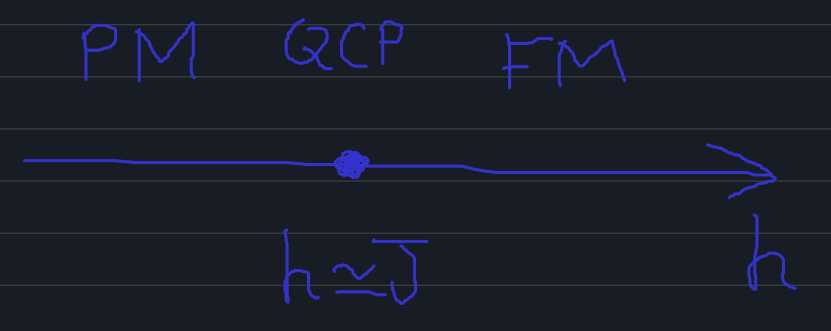
\includegraphics[width=0.75\textwidth]{fig/qcp.png}
\caption{Diagrama de fase com transição de fase quântica em $T = 0$.}
\label{fig:qcp}
\end{figure}


\n

(b) Com as transformações de Jordan-Wigner
$$
\s_j^z = 1 - 2 n_j,
$$
$$
\s_j^x = \qty[\prod_{k < j} (1-2n_k)] (c_j + c_j^\d),
$$
temos que a hamiltoniana de Ising 1D em campo transverso se escreve
$$
H = -J \sum_{j} \s_j^x \s_{j+1}^x - h \sum_{j} \s_j^z =
-J \sum_{j} \qty[\prod_{k<j} (1 - 2n_k)^2] (c_j+c_j^\d)(1-2n_j)(c_{j+1} + c_{j+1}^\d) - h \sum_{j} (1-2n_j).
$$

Veja que $(1-2n_k)^2 = 1 - 4 n_k + 4 n_k^2 = 1$. Como $(c_j+c_j^\d)(1-2n_j) = c_j^\d - c_j$, temos
\begin{equation} \label{eq:hamil_transvising}
H = -J \sum_{j} \qty[ c_j^\d c_{j+1} + c_{j+1} c_j + \hc ]
+ 2h \sum_{j} c_j^\d c_j - h \sum_{j} 1.
\end{equation}

Tomando agora as transformadas $c_j = \frac{1}{\sqrt{N}} \sum_{k} e^{ikj} c_k$:
$$
H =
-\frac{J}{N} \sum_{j} \sum_{k,k'} \qty[ e^{ik'} e^{-i(k-k')j} c_k^\d c_{k'} + e^{ik'} e^{i(k+k')j} c_{k'} c_k + \hc ]
+ 2h \sum_{k} c_k^\d c_k - h N.
$$
$$
H =
-J \sum_{k} \qty[ e^{ik} c_k^\d c_{k} + e^{-ik} c_{-k} c_k + \hc ]
+ h \sum_{k} (c_k^\d c_k - c_{-k} c_{-k}^\d).
$$
$$
H =
\frac{1}{2}
\sum_{k}
\begin{pmatrix}
c_k^\d & c_{-k}
\end{pmatrix}
\begin{pmatrix}
2(h - J \cos k) & -2iJ \sin k \\
2iJ \sin k & -2(h - J\cos k)
\end{pmatrix}
\begin{pmatrix}
c_k \\ c_{-k}^\d
\end{pmatrix}
+ \cte.
$$

É imediato que os autovalores são $\omega(k) = \pm 2\sqrt{J^2 + h^2 - 2hJ \cos k}$. A transformação de Bogoliubov que diagonaliza a hamiltoniana é
$$
\begin{pmatrix}
c_k \\ c_{-k}^\d
\end{pmatrix}
=
\begin{pmatrix}
 \cos \theta_k & i\sin \theta_k  \\
i\sin \theta_k &  \cos \theta_k
\end{pmatrix}
\begin{pmatrix}
a_k \\ a_{-k}^\d
\end{pmatrix},
$$
e fazendo as contas, descobre-se que $\tan(2\theta_k) = \frac{J \sin k}{h - J \cos k}$.

\begin{figure}[H]
\centering
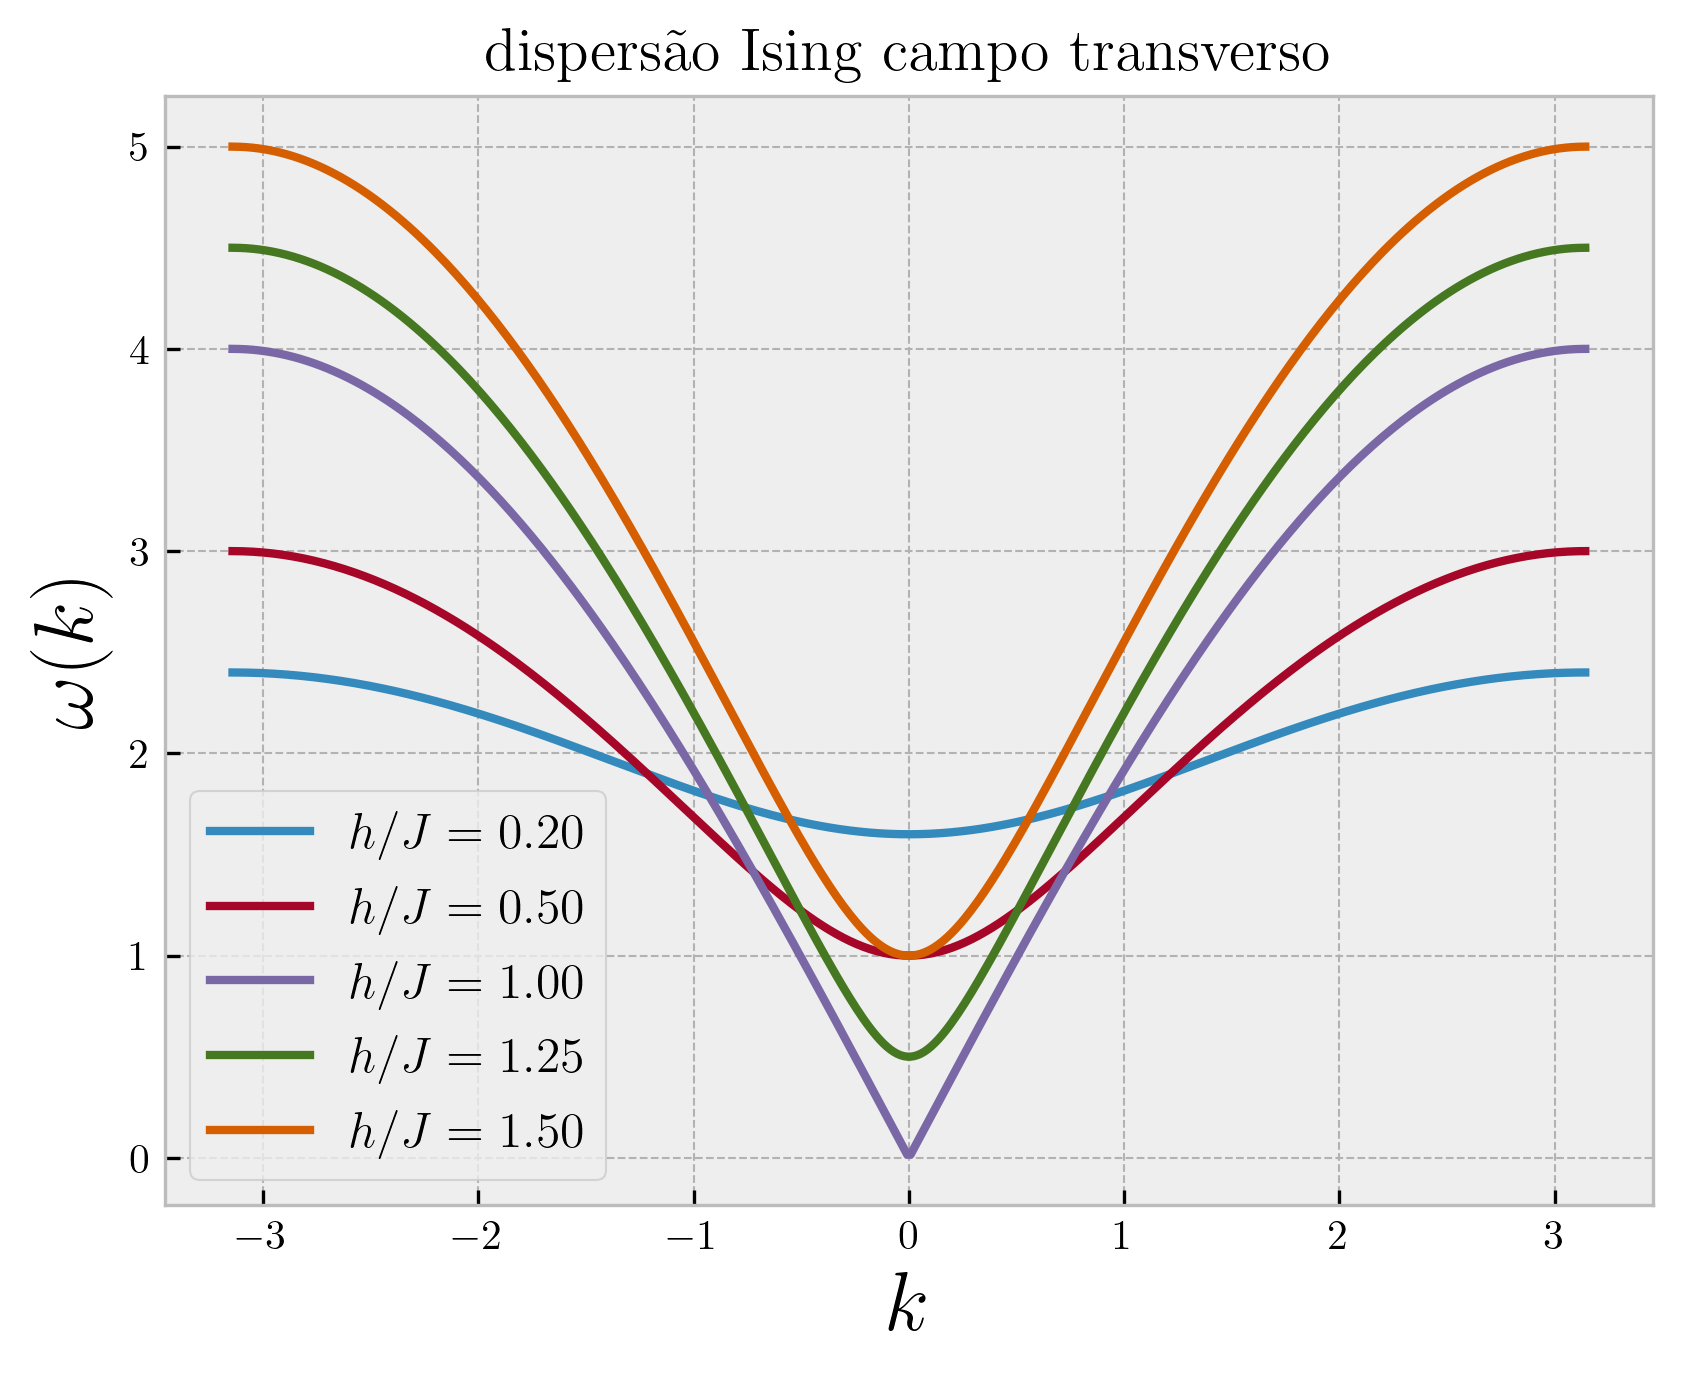
\includegraphics[width=0.5\textwidth]{fig/transv_ising.png}
\caption{Dispersão $\omega(k) = 2\sqrt{J^2 + h^2 - 2hJ \cos k}$ para várias razões $h/J$. Vemos que para $h/J = 1$ a curva forma um cone (fecha o gap).}
\label{fig:transv_ising}
\end{figure}

Olhando para a Figura \ref{fig:transv_ising}, podemos identificar que a transição de fase quântica ocorre quando $h/J = 1$, que é o valor em que a dispersão forma um cone em torno de $k = 0$ (fechamento do gap).

\n

A magnetização é dada por
$$
m_z = \frac{1}{N} \sum_{j} \ev{\s_j^z} = 2 \frac{1}{N}\sum_{k} \ev{c_k^\d c_k} - 1.
$$

Pela transformação de Bogoliubov tem-se
$$
c_k^\d c_k = \cos[2](\theta_k) a_k^\d a_k + \sin[2](\theta_k) a_{-k}a_{-k}^\d
+ i \sin\theta_k \cos\theta_k (a_{k}^\d a_{-k}^\d - a_{-k} a_{-k})
$$

Para $T = 0$ temos que $\ev{X} = \ev{X}{0}$ e que $a_k \ket{0} = 0$. Portanto $\ev{c_k^\d c_k} = \sin[2](\theta_k)$. Usando que $2 \sin[2](x) = \frac{\tan[2](2x)}{1 + \tan[2](2x)}$, obtemos que
$$
m_z + 1 = \int_{-\pi}^{\pi} \frac{J^2 \sin[2](k)}{[h-J\cos(k)]^2 + J^2\sin[2](k)} \dd{k}.
$$
Pedindo para o Mathematica resolver a integral acima, ele retorna
$$
m_z + 1 =
\begin{cases}
\; \pi \frac{J^2}{h^2} , \quad h/J \geq 1, \\
\; \pi , \quad \quad \, h/J < 1. \\
\end{cases}
$$

Acho que o resultado acima não faz sentido né... Mas não sei como consertar.

\n

(d) O hamiltoniano de Kitaev é
$$
H = -t \sum_{i} (c_{i+1}^\d c_i + \hc) - \mu \sum_{i} c_i^\d c_i
+ \Delta \sum_{i} (c_{i+1}^\d c_i^\d + \hc).
$$

É fácil ver que a hamiltoniana do Ising transverso \ref{eq:hamil_transvising} é um caso particular do Kitaev para $\Delta = -J$, $t = J$ e $\mu = -2h$. Como podemos ver em \url{https://topocondmat.org/w1_topointro/1D.html}, para o modelo de Kitaev, a fase trivial acontece para $\abs{\mu} < 2t$ e a topológica para $\abs{\mu} > 2t$. Essas duas fases correspondem à paramagnética e ferromagnética do Ising transversal, respectivamente.


\pagebreak


\section{Teoria de Lindemann para o derretimento de um cristal}

\textbf{Vou deixar essa passar...}



\pagebreak


\section{Tamanho do par de Cooper}

(a) Estimamos $\Delta E \approx \Delta_0$ e $\Delta x \approx v_F \Delta t$, com $v_F = \hbar k_F / m_e = (\hbar/m_e) (3\pi^2 n)^{1/3}$ para elétrons livres em 3D. Assim
$$
\Delta x \approx
\frac{v_F}{\Delta E} \cdot \overbrace{(\Delta E \Delta t)}^{\hbar}
\approx \frac{\hbar^2}{m_e \Delta_0} (3\pi^2 n)^{1/3}.
$$

Utilizando a relação para o gap $\Delta_0 = 1.764 \cdot k_B T_c$

\n\n

(b) Olhando nas tabelas 1.1 e 34.2 do Ashcroft temos para o alumínio (Al) $n = 1.81 \times 10^{23} \unit{cm^{-3}}$ e $T_c = 1.196 \unit{K}$, respectivamente.

\n

Usando os valores $k_B = 1.38 \times 10^{-23} \unit{J \cdot K^{-1}}$, $\hbar = 1.055 \times 10^{-34} \unit{J \cdot s}$ e $m_e = 9.109 \times 10^{-31} \unit{kg}$, obtemos
$$
\boxed{ \Delta x \approx 7 \unit{\mu m}. }
$$

\pagebreak


\section{Termodinâmica BCS}

(a) Das notas de aula, partimos da equação do gap
$$
1 = \frac{g_0}{V} \sum_{\k} \frac{1}{2 E_{\k}} \tanh(\frac{\beta E_{\k}}{2})
\simeq
2 g_0 \, N(E_F) \int_0^{\hbar \omega_D} \dd{\eps}
\frac{\tanh(\frac{\beta}{2} \sqrt{\eps^2 + \abs{\Delta(T)}^2})}
{2 \sqrt{\eps^2 + \abs{\Delta(T)}^2}}.
$$

Fazendo $T \to T_c$ ($\beta \to \beta_c)$, temos que $\Delta \to 0$. Assim ficamos com
$$
1 = g_0 N(E_F) \int_0^{\beta_c \hbar \omega_D / 2} \frac{\tanh x}{x} \dd{x}.
$$

O truque para avaliar a integral acima analiticamente é integração por partes:
$$
\int_0^{\beta_c \hbar \omega_D / 2} \frac{\tanh x}{x} \dd{x} =
\eval{\qty(\ln x \tanh x)}_{0}^{\beta_c \hbar \omega_D / 2} -
\int_0^{\beta_c \hbar \omega_D / 2} \frac{\ln x}{\cosh[2](x)} \dd{x}.
$$

Agora supondo que $1/\beta_c = k_B T_c \ll \hbar \omega_D$, aproximamos a tangente hiperbólica por 1 e substituimos o limite superior de integração para infinito:
$$
\int_0^{\beta_c \hbar \omega_D / 2} \frac{\tanh x}{x} \dd{x} =
\ln (\frac{\hbar \omega_D}{2 k_B T_c}) -
\int_0^{\infty} \frac{\ln x}{\cosh[2](x)} \dd{x}.
$$

Pedindo para o Mathematica calcular a integral imprópria, eles nos retorna
$$
\int_0^{\infty} \frac{\ln x}{\cosh[2](x)} \dd{x} =
- \gamma + \ln(\frac{\pi}{4}),
$$
onde $\displaystyle{\gamma \equiv \lim_{n \to \infty} \qty(-\log n + \sum_{k=1}^{n} \frac{1}{k})} \simeq 0.57721$ é a constante de Euler-Mascheroni. Dessa maneira, obtemos
$$
-\frac{1}{g_0 N(E_F)} = \ln (\frac{2 k_B T_c}{\hbar \omega_D})
- \gamma + \ln(\frac{\pi}{4}) \implies
$$
$$
\boxed{ k_B T_c = \frac{2 e^{\gamma}}{\pi}
\cdot \hbar \omega_D e^{-\frac{1}{g_0 N(E_F)}} =
1.13387 \cdot \hbar \omega_D e^{-\frac{1}{g_0 N(E_F)}}. }
$$

Nas aulas vimos que $\Delta_0 = 2 \hbar \omega_D e^{-\frac{1}{g_0 N(E_F)}}$. Portanto a razão
$$
\frac{\Delta_0}{k_B T_c} = \frac{\pi}{e^{\gamma}} \simeq 1.76388
$$
é um número universal.

\n

(b) Para uma densidade de estados constante integrar a 1, temos que $N(\eps) = \frac{1}{\hbar \omega_D}$. Calculamos o gap numericamente definindo a função
$$
\vphi_T(\Delta) =
1 - g_0 N(E_F) \int_{0}^{\hbar \omega_D} \dd{\eps}
\frac{\tanh(\frac{1}{2T} \sqrt{\eps^2 + \Delta^2})}
{\sqrt{\eps^2 + \Delta^2}},
$$
e extraindo suas raízes para cada $T$.

\begin{figure}[H]
\centering
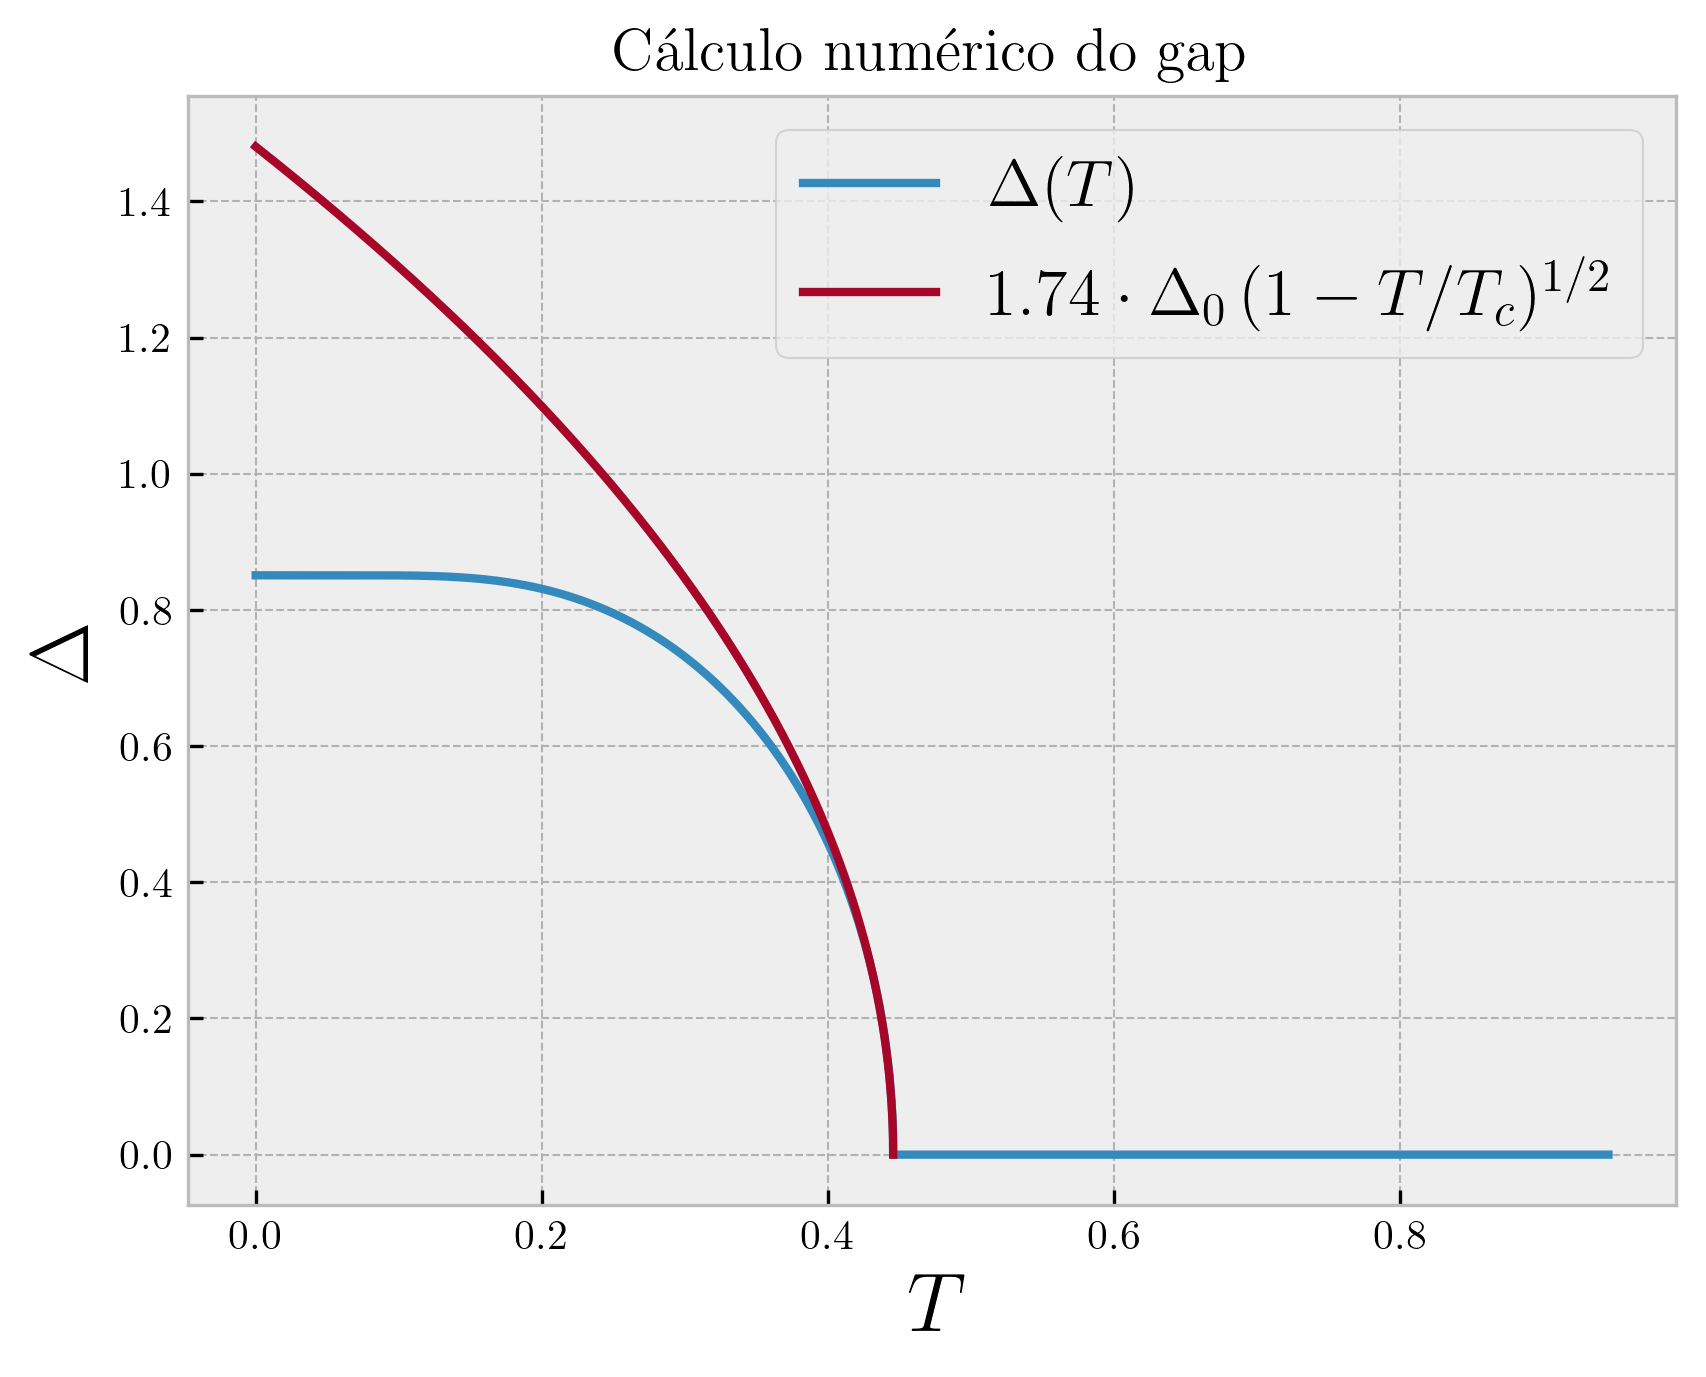
\includegraphics[width=0.6\textwidth]{fig/num_gap.png}
\caption{Cálculo numérico de $\Delta(T)$, com parâmetros $k_B = g_0 = \hbar \omega_D = 1$. Neste caso $T_c = 0.4456$ e obtive a razão $\Delta_0 / T_c = 1.91$.}
\label{fig:num_gap}
\end{figure}

\n

Na Figura \ref{fig:num_gap}, vemos que a aproximação $\Delta(T) / \Delta_0 = 1.74 (1 - T/T_c)^{1/2}$ é compatível para valores $T \to T_c$. Isso mostra que o expoente crítico para o gap realmente é $1/2$, assim como a teoria de Landau prevê.

\n

Penso que a teoria de campo médio descreve bem os experimentos para supercondutores BCS pois os elétrons dos pares de Cooper interagem à longuíssimos alcances, de maneira que a aproximação de um campo médio se torna muito boa.

\n

(c) Utilizando a entropia de Shannon para um gás de férmions (partícula ou buraco para cada estado $\k$) com dispersão $E_{\k} = \sqrt{\eps_{\k}^2 + \Delta^2}$, temos
$$
S = - k_B \sum_{\k}
\qty[
f_{\k} \ln f_{\k} + (1 - f_{\k}) \ln(1 - f_{\k})
],
$$
onde $f_{\k} = \frac{1}{e^{\beta E_{\k}} + 1}$ é a distribuição de Fermi-Dirac. Omitindo passos algébricos, o calor específico é então dado por
$$
C = -\beta \pdv{S}{\beta} = - k_B \beta \sum_{\k} \dv{f}{E_{\k}}
\qty[E_{\k}^2 + \beta \Delta \pdv{\Delta}{\beta}] =
2 k_B \beta N(E_F)
\int_0^{\hbar \omega_D} \qty(-\pdv{f}{E})
\qty(E^2 + \beta \Delta \dv{\Delta}{\beta}) \dd{\eps}.
$$

Para $T \to 0$ temos que $f \simeq e^{-\beta E}$, $\dv{\Delta}{\beta} \simeq 0$ e $E \simeq \Delta_0$. Portanto
$$
C = 2 k_B \beta^2 N(E_F) \Delta_0^2 \hbar \omega_D e^{-\beta \Delta_0} \propto
e^{-\Delta_0 / k_B T}.
$$

\end{document}
